In this chapter we conduct two experiments to demonstrate that our proposed method outperforms other traditional methods that have been introduced in previous chapters. The implementation is available at the website xxxx.

\section{Dataset}

We collected data of 524 instances of a single-leg drop jump landing from 144 college football (soccer) players from the University of Tsukuba.
\\

The dataset consists of the following attributes:
\begin{itemize}
	\item 3 dimensional coordinates of 29 body markers capture by multiple infrared cameras. A full list of the where the body markers where place is available in Table \ref{body_markers}.
	\item An integer (1~9) indicating the classification of ankle instability, labelled by an expert (label description: 1=Healthy, 2=Structural instability, 3=Subjective instability, 4=Sprained more than 3 times, 5=2 and 3, 6=2 and 4, 7=3 and 4, 8=2 and 3 and 4, 9=healthy but with a history of one or two sprains).
	\item Binary labels (0 or 1) indicating classes. For example, whether the single-leg drop jump was successful (0) or not (1). After consolation with an expert, we defined a successful jump as a jump where the subject was able to keep their balance on a single leg for more than 5 seconds after landing. A full list of the binary labels are available in Table \ref{binary_labels}.
	\item Force plate data.
	\item Weight (kg) for each of the individual 144 athletes.
\end{itemize}

\begin{table}[!h]
	\centering
	\begin{tabular}{p{0.35\linewidth} | p{0.6\linewidth}}
		\textbf{Label~}        & \textbf{Explanation}                                                                                  \\ \hline
		Success                & 0 if the subject can balance on one foot for 5 seconds after SDJ, otherwise 1                         \\ \hline
		Jump Leg               & 0 if subject jumped with right foot, otherwise 1                                                      \\ \hline
		Healthy                & 0 if ll of the below are 0, otherwise 1                                                              \\ \hline
		Prior Injury           & 0 if subject has no previous injuries, otherwise 1                                                    \\ \hline
		Structural Instability & 0 if expert determines that the joint is loose due to ligament damage after palpation, otherwise 1    \\ \hline
		Subjective Instability & 0 if the subject is determined to have instability in the ankle joint by a questionnaire, otherwise 1 \\ \hline
		Prone                  & 1 if the subject has 1 or more sprains and none of the above three labels are 1, otherwise 0          \\ \hline
	\end{tabular}
	\caption{List of binary labels}
	\label{binary_labels}
\end{table}


% % Please add the following required packages to your document preamble:
% % \usepackage[normalem]{ulem}
% % \useunder{\uline}{\ul}{}
\begin{table}[!h]
	\centering
	\begin{tabular}{|c|l|}
		\hline
		{\ul \textbf{Index}} & \multicolumn{1}{c|}{{\ul \textbf{Name}}} \\ \hline
		0                    & Cervical vertebra 7                      \\ \hline
		1                    & Calcaneal tuberosity                     \\ \hline
		2                    & Fibula Head                              \\ \hline
		3                    & Greater trochanter                       \\ \hline
		4                    & Suprasternal notch                       \\ \hline
		5                    & Anterior superior iliac spine (L)        \\ \hline
		6                    & lateral epicondyle                       \\ \hline
		7                    & medial malleolus                         \\ \hline
		8                    & Posterior superior iliac spine (L)       \\ \hline
		9                    & medial condyle                           \\ \hline
		10                   & medial epicondyle                        \\ \hline
		11                   & lateral malleolus                        \\ \hline
		12                   & Base of first metatarsal bone            \\ \hline
		13                   & Base of second metatarsal bone           \\ \hline
		14                   & Base of fifth metatarsal bone            \\ \hline
		15                   & Head of first metatarsal bone            \\ \hline
		16                   & Head of second metatarsal bone           \\ \hline
		17                   & Head of fifth metatarsal bone            \\ \hline
		18                   & Fibular trochlea of calcaneus            \\ \hline
		19                   & First distal phalanges                   \\ \hline
		20                   & Anterior superior iliac spine (R)        \\ \hline
		21                   & Posterior superior iliac spine (L)       \\ \hline
		22                   & Acromion (L)                             \\ \hline
		23                   & Acromion (R)                             \\ \hline
		24                   & Sustentaculum tali                       \\ \hline
		25                   & Thoracic vertebrae 8                     \\ \hline
		26                   & Tibial tuberosity                        \\ \hline
		27                   & Scaphoid bone                            \\ \hline
		28                   & Xiphoid process                          \\ \hline
	\end{tabular}
	\caption{List of body markers}
	\label{body_markers}
\end{table}

% 上記に加え,15名分の6.片脚着地動作時の多視点映像を用いて平面撮像のみでの評価可能性の検証を行う.
% 倫理審査に先行して,サンプルデータ(N=40)を入手.サンプルデータは,体表マーカーの3次元座標データ・成功失敗の2値ラベル・着地の良し悪しの2値ラベル・床反力Fz最大値・床反力Fz最大値出現時間(ms)・衝撃吸収能力がセットとなっている.それぞれについて以下に詳細を示す.

% \subsection{体表マーカーの3次元座標データ}

\newpage
%================================================================
% * New page
%================================================================

\begin{figure}[!hb]
	\centering
	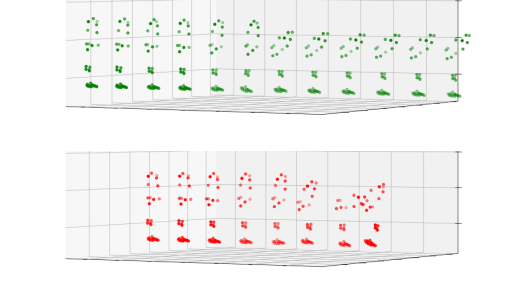
\includegraphics{images/sample_sequence.png}
	\caption{Two jump sequences sampled at 1fps. The successful jump is colored in green and the unsuccessful jump is colored in red.}
	\label{figure:sample sequence}
\end{figure}

% \import{images/}{coordinate_hist.tex}
% \import{tables/}{pose_description.tex}

% \subsection{ラベルデータ}
% \import{images/}{label_correlation.tex}
% \import{tables/}{label_description.tex}

\section{Evaluation Metrics}

To evaluate the performance of different classification methods, we use a 5-fold cross-validation strategy to compute the classification accuracy, F1 score and the area under the receiver operating characteristic curve (AUC).

Although accuracy is a sufficient metric for performance in datasets with symmetric classes distribution and class value, it is an inadequate metric for datasets with class imbalance and datasets where values of false positive and false negatives are differ.

Therefore, we included the two additional metrics explained above. These metrics are frequently used in medical cases such as cancer detection from images \cite{Sirinukunwattana2016LocalityImages}\cite{Ciresan2013MitosisNetworks}.

\subsection{Accuracy}
Accuracy is computed as the fraction of correct predictions.

\[ \texttt{accuracy}(y, \hat{y}) = \frac{1}{n_\text{samples}} \sum_{i=0}^{n_\text{samples}-1} 1(\hat{y}_i = y_i) \]

\subsection{F1 Score}
The F1 score can be interpreted as an average of the classifier’s ability to:
\begin{itemize}
	\item Not label as negative samples as a positive (i.e. Precision).
	\item Find all positive samples (i.e. Recall).
\end{itemize}

\[ F_1 = 2 \times \frac{\text{precision} \times \text{recall}}{\text{precision} + \text{recall}} \]

\subsection{Area Under the Curve}
The receiver operating characteristic (ROC) plots the true positive rate (TPR) to the false positive rate (FPR) of a binary classifier with varying discrimination thresholds.

The area under the ROC curve (AUC) summarizes the information of the ROC in one number, between 0 and 1. AUC = 0.5 indicates an uniformative classifier (a classifier with uniform prediction for any sample) or random classifier if the classes are symmetric. Therefore no realistic classifiershould have an AUC $<$ 0.5. AUC = 1 indicates a perfect classifier.

The algorithm to compute AUC with an in-depth explanation can be found in \cite{Fawcett2006AnAnalysis}.

\section{Experiment 1.}
In this experiment we evaluate x classifiers accuracy on multiple binary classification problems regarding our single-leg drop jump dataset.

\subsection{Experiment setup}
We experiment with the following setup.

\begin{enumerate}[label=(\Alph*)]
	\item Pose data up until landing.
	\item All pose data.
	\item Pose data + Force Plate data.
\end{enumerate}

\subsection{Results}
\subsection{}

% \subsection{足関節不安定症の病態分類}
% 未取得
% \subsection{片脚着地動作時の床反力データ}
% 未取得
% \subsection{個人情報(年齢・身長・体重・ポジション・利き足・筑波大学蹴球部(男子)内の所属チーム)}
% 未取得
% \subsection{エキスパート(医者・トレーナー)による着地動作の良し悪しのラベル}
% 未取得